% Options for packages loaded elsewhere
\PassOptionsToPackage{unicode}{hyperref}
\PassOptionsToPackage{hyphens}{url}
%
\documentclass[
  ignorenonframetext,
  aspectratio=169,
]{beamer}
\usepackage{pgfpages}
\setbeamertemplate{caption}[numbered]
\setbeamertemplate{caption label separator}{: }
\setbeamercolor{caption name}{fg=normal text.fg}
\beamertemplatenavigationsymbolsempty
% Prevent slide breaks in the middle of a paragraph
\widowpenalties 1 10000
\raggedbottom
\setbeamertemplate{part page}{
  \centering
  \begin{beamercolorbox}[sep=16pt,center]{part title}
    \usebeamerfont{part title}\insertpart\par
  \end{beamercolorbox}
}
\setbeamertemplate{section page}{
  \centering
  \begin{beamercolorbox}[sep=12pt,center]{part title}
    \usebeamerfont{section title}\insertsection\par
  \end{beamercolorbox}
}
\setbeamertemplate{subsection page}{
  \centering
  \begin{beamercolorbox}[sep=8pt,center]{part title}
    \usebeamerfont{subsection title}\insertsubsection\par
  \end{beamercolorbox}
}
\AtBeginPart{
  \frame{\partpage}
}
\AtBeginSection{
  \ifbibliography
  \else
    \frame{\sectionpage}
  \fi
}
\AtBeginSubsection{
  \frame{\subsectionpage}
}

\usepackage{amsmath,amssymb}
\usepackage{iftex}
\ifPDFTeX
  \usepackage[T1]{fontenc}
  \usepackage[utf8]{inputenc}
  \usepackage{textcomp} % provide euro and other symbols
\else % if luatex or xetex
  \usepackage{unicode-math}
  \defaultfontfeatures{Scale=MatchLowercase}
  \defaultfontfeatures[\rmfamily]{Ligatures=TeX,Scale=1}
\fi
\usepackage{lmodern}
\ifPDFTeX\else  
    % xetex/luatex font selection
\fi
% Use upquote if available, for straight quotes in verbatim environments
\IfFileExists{upquote.sty}{\usepackage{upquote}}{}
\IfFileExists{microtype.sty}{% use microtype if available
  \usepackage[]{microtype}
  \UseMicrotypeSet[protrusion]{basicmath} % disable protrusion for tt fonts
}{}
\makeatletter
\@ifundefined{KOMAClassName}{% if non-KOMA class
  \IfFileExists{parskip.sty}{%
    \usepackage{parskip}
  }{% else
    \setlength{\parindent}{0pt}
    \setlength{\parskip}{6pt plus 2pt minus 1pt}}
}{% if KOMA class
  \KOMAoptions{parskip=half}}
\makeatother
\usepackage{xcolor}
\newif\ifbibliography
\setlength{\emergencystretch}{3em} % prevent overfull lines
\setcounter{secnumdepth}{-\maxdimen} % remove section numbering


\providecommand{\tightlist}{%
  \setlength{\itemsep}{0pt}\setlength{\parskip}{0pt}}\usepackage{longtable,booktabs,array}
\usepackage{calc} % for calculating minipage widths
\usepackage{caption}
% Make caption package work with longtable
\makeatletter
\def\fnum@table{\tablename~\thetable}
\makeatother
\usepackage{graphicx}
\makeatletter
\def\maxwidth{\ifdim\Gin@nat@width>\linewidth\linewidth\else\Gin@nat@width\fi}
\def\maxheight{\ifdim\Gin@nat@height>\textheight\textheight\else\Gin@nat@height\fi}
\makeatother
% Scale images if necessary, so that they will not overflow the page
% margins by default, and it is still possible to overwrite the defaults
% using explicit options in \includegraphics[width, height, ...]{}
\setkeys{Gin}{width=\maxwidth,height=\maxheight,keepaspectratio}
% Set default figure placement to htbp
\makeatletter
\def\fps@figure{htbp}
\makeatother
\newlength{\cslhangindent}
\setlength{\cslhangindent}{1.5em}
\newlength{\csllabelwidth}
\setlength{\csllabelwidth}{3em}
\newlength{\cslentryspacingunit} % times entry-spacing
\setlength{\cslentryspacingunit}{\parskip}
\newenvironment{CSLReferences}[2] % #1 hanging-ident, #2 entry spacing
 {% don't indent paragraphs
  \setlength{\parindent}{0pt}
  % turn on hanging indent if param 1 is 1
  \ifodd #1
  \let\oldpar\par
  \def\par{\hangindent=\cslhangindent\oldpar}
  \fi
  % set entry spacing
  \setlength{\parskip}{#2\cslentryspacingunit}
 }%
 {}
\usepackage{calc}
\newcommand{\CSLBlock}[1]{#1\hfill\break}
\newcommand{\CSLLeftMargin}[1]{\parbox[t]{\csllabelwidth}{#1}}
\newcommand{\CSLRightInline}[1]{\parbox[t]{\linewidth - \csllabelwidth}{#1}\break}
\newcommand{\CSLIndent}[1]{\hspace{\cslhangindent}#1}


% DELETED!
% DELETED!
% DELETED!
% DELETED!
% DELETED!

% DELETED!
\newcommand{\sufstats}[1]{\bm{g}\left(#1\right)}
\renewcommand{\exp}[1]{\mbox{exp}\left\{#1\right\}}
\renewcommand{\log}[1]{\mbox{log}\left\{#1\right\}}
\newcommand{\transpose}[1]{{#1}^{\bm{t}}} 
\renewcommand{\t}[1]{\transpose{#1}}

\newcommand{\s}[1]{\sufstats{#1}}
\newcommand{\SUFF}{\bm{S}}
\newcommand{\Suff}{\bm{G}}
\newcommand{\suff}{\bm{g}}

\newcommand{\coef}{\bm{\theta}}
\newcommand{\weight}{\bm{w}}
\newcommand{\Weight}{\bm{W}}

% Objects
% DELETED!
% DELETED!
\newcommand{\Graph}{\bm{Y}}
\newcommand{\graph}{\bm{y}}
\newcommand{\g}{\graph}
\newcommand{\GRAPH}{\mathcal{Y}}
\newcommand{\Adjmat}{A}
\newcommand{\adjmat}{a}
\newcommand{\ADJMAT}{\bm{A}}

\newcommand{\INDEPVAR}{\bm{X}}
\newcommand{\Indepvar}{X}
\newcommand{\indepvar}{x}

\newcommand{\normconst}{\kappa_{\GRAPH}\left(\coef\right)}


% \bibliography{bibliography.bib}

\def\ergmito{ERGM\textit{ito}}
\def\ergmitos{\ergmito{}\textit{s}}
% Mathematical functions
\newcommand{\isone}[1]{{\boldsymbol{1}\left( #1 \right)}}
\newcommand{\f}[1]{{f\left(#1\right) }}

% Define a command with an optional argument

% \usepackage[]{xparse}
% \NewDocumentCommand{\Prcond}{m m o}{
%   \IfNoValueTF{#3}{%
%   {\mbox{Pr}\left(#1;\;#2\right)} %
%   }{%
%   {\mbox{Pr}_{#3}\left(#1;\;#2\right)} %
%   }
% }

\renewcommand{\Pr}[1]{{\mbox{Pr}_{\GRAPH,\coef}\left(#1\right) }}
\newcommand{\Prcond}[2]{%
  {\mbox{Pr}_{\GRAPH,\coef}\left(#1\left|\;#2\right.\right)}%
  }
\newcommand{\fcond}[2]{{f\left(#1|#2\right) }}
\newcommand{\Expected}[1]{{\mathbb{E}\left\{#1\right\}}}
\newcommand{\ExpectedCond}[2]{{\mathbb{E}\left\{#1\vphantom{#2}\right|\left.\vphantom{#1}#2\right\}}}
\renewcommand{\exp}[1]{\mbox{exp}\left\{#1\right\}}

\newcommand{\Likelihood}[2]{\text{L}\left(#1 \left|\vphantom{#1}#2\right.\right)}

\newcommand{\loglik}[1]{l\left(#1\right)}
\makeatletter
\makeatother
\makeatletter
\makeatother
\makeatletter
\@ifpackageloaded{caption}{}{\usepackage{caption}}
\AtBeginDocument{%
\ifdefined\contentsname
  \renewcommand*\contentsname{Table of contents}
\else
  \newcommand\contentsname{Table of contents}
\fi
\ifdefined\listfigurename
  \renewcommand*\listfigurename{List of Figures}
\else
  \newcommand\listfigurename{List of Figures}
\fi
\ifdefined\listtablename
  \renewcommand*\listtablename{List of Tables}
\else
  \newcommand\listtablename{List of Tables}
\fi
\ifdefined\figurename
  \renewcommand*\figurename{Figure}
\else
  \newcommand\figurename{Figure}
\fi
\ifdefined\tablename
  \renewcommand*\tablename{Table}
\else
  \newcommand\tablename{Table}
\fi
}
\@ifpackageloaded{float}{}{\usepackage{float}}
\floatstyle{ruled}
\@ifundefined{c@chapter}{\newfloat{codelisting}{h}{lop}}{\newfloat{codelisting}{h}{lop}[chapter]}
\floatname{codelisting}{Listing}
\newcommand*\listoflistings{\listof{codelisting}{List of Listings}}
\makeatother
\makeatletter
\@ifpackageloaded{caption}{}{\usepackage{caption}}
\@ifpackageloaded{subcaption}{}{\usepackage{subcaption}}
\makeatother
\makeatletter
\@ifpackageloaded{tcolorbox}{}{\usepackage[skins,breakable]{tcolorbox}}
\makeatother
\makeatletter
\@ifundefined{shadecolor}{\definecolor{shadecolor}{rgb}{.97, .97, .97}}
\makeatother
\makeatletter
\makeatother
\makeatletter
\makeatother
\makeatletter
\@ifpackageloaded{fontawesome5}{}{\usepackage{fontawesome5}}
\makeatother
\ifLuaTeX
  \usepackage{selnolig}  % disable illegal ligatures
\fi
\IfFileExists{bookmark.sty}{\usepackage{bookmark}}{\usepackage{hyperref}}
\IfFileExists{xurl.sty}{\usepackage{xurl}}{} % add URL line breaks if available
\urlstyle{same} % disable monospaced font for URLs
\hypersetup{
  pdftitle={Power and multicollinearity in small networks: A discussion of},
  pdfauthor={George G. Vega Yon, Ph.D.},
  hidelinks,
  pdfcreator={LaTeX via pandoc}}

\title{Power and multicollinearity in small networks: A discussion of}
\subtitle{``Tale of Two Datasets: Representativeness and
Generalisability of Inference for Samples of Networks''JSM 2023Toronto,
Canada}
\author{George G. Vega Yon, Ph.D.}
\date{2023-06-28}
\institute{The University of Utah}

\begin{document}
\frame{\titlepage}
\ifdefined\Shaded\renewenvironment{Shaded}{\begin{tcolorbox}[boxrule=0pt, breakable, interior hidden, sharp corners, borderline west={3pt}{0pt}{shadecolor}, frame hidden, enhanced]}{\end{tcolorbox}}\fi

\hypertarget{overview}{%
\section{Overview}\label{overview}}

\begin{frame}{Highlights Krivitsky, Coletti, and Hens (2022)}
\protect\hypertarget{highlights-krivitskytaletwodatasets2022}{}
What I highlight in their paper:

\begin{itemize}
\item
  Start to finish framework for multi-ERG models.
\item
  Dealing with heterogeneous samples.
\item
  Model building process.
\item
  Goodness-of-fit analyses.
\end{itemize}

Two important missing pieces (for the next paper): power analysis and
how to deal with collinearity in small networks.
\end{frame}

\hypertarget{power-analysis-in-ergms}{%
\section{Power analysis in ERGMs}\label{power-analysis-in-ergms}}

\begin{frame}{Sample size in ERGMs}
\protect\hypertarget{sample-size-in-ergms}{}
Two different questions: \emph{How many nodes?} and ``\emph{How many
networks?}''

\begin{block}{Number of nodes}
\protect\hypertarget{number-of-nodes}{}
\begin{itemize}
\item
  Is the network bounded?
\item
  If it is bounded, can we collect all the nodes?
\item
  If we cannot collect all the nodes, can we do inference
  (Schweinberger, Krivitsky, and Butts 2017; Schweinberger et al. 2020)?
\end{itemize}
\end{block}

\begin{block}{Number of networks}
\protect\hypertarget{number-of-networks}{}
\begin{itemize}
\item
  There is a growing number of studies featuring multiple networks
  (e.g., egocentric studies).
\item
  There's no clear way to do power analysis in ERGMs.
\item
  In funding justification, power analysis is fundamental, so we need
  that.
\end{itemize}
\end{block}
\end{frame}

\begin{frame}{A possible approach}
\protect\hypertarget{a-possible-approach}{}
We can leverage conditional ERG models for power analysis.

\begin{itemize}
\item
  Conditioning on one sufficient statistic results in a distribution
  invariant to the associated parameter, formally:

  \begin{align}
  \notag%
    {\mbox{Pr}_{\mathcal{Y},\boldsymbol{\theta}}\left(\boldsymbol{Y}= \boldsymbol{y}\left|\;\boldsymbol{g}\left(\boldsymbol{y}\right)_l = s_l\right.\right)}%
      & = \frac{%
    {\mbox{Pr}_{\mathcal{Y},\boldsymbol{\theta}}\left(\boldsymbol{g}\left(\boldsymbol{Y}\right)_{-l} = \boldsymbol{g}\left(\boldsymbol{y}\right)_{-l}, \boldsymbol{g}\left(\boldsymbol{y}\right)_l = s_l\right) }
  }{%
    \sum_{\boldsymbol{y}'\in\mathcal{Y}:\boldsymbol{g}\left(\boldsymbol{y}'\right)_l = s_l}{\mbox{Pr}_{\mathcal{Y},\boldsymbol{\theta}}\left(\boldsymbol{g}\left(\boldsymbol{Y}\right) = \boldsymbol{y}'\right) }%
  } \\ & =  %
  \frac{%
    \mbox{exp}\left\{{\boldsymbol{\theta}_{-l}}^{\boldsymbol{t}}\boldsymbol{g}\left(\boldsymbol{y}\right)_{-l}\right\}
  }{%
    \kappa_{\mathcal{Y}}\left(\boldsymbol{\theta}\right)_{-l}
  }, \tag{1}
  \end{align}

  where \(\boldsymbol{g}\left(\boldsymbol{y}\right)_l\) and
  \(\boldsymbol{\theta}_l\) are the \(l\)-th element of
  \(\boldsymbol{g}\left(\boldsymbol{y}\right)\) and
  \(\boldsymbol{\theta}\) respectively,
  \(\boldsymbol{g}\left(\boldsymbol{y}\right)_{-l}\) and
  \(\boldsymbol{\theta}_{-l}\) are their complement, and
  \(\kappa_{\mathcal{Y}}\left(\boldsymbol{\theta}\right)_{-l} = \sum_{\boldsymbol{y}' \in \mathcal{Y}: \boldsymbol{g}\left(\boldsymbol{y}'\right)_l = s_l}\mbox{exp}\left\{{\boldsymbol{\theta}_{-l}}^{\boldsymbol{t}}\boldsymbol{g}\left(\boldsymbol{y}'\right)_{-l}\right\}\)
  is the normalizing constant.
\item
  We can use this to generate networks with a prescribed density (based
  on previous studies) and compute power through simulation.
\end{itemize}
\end{frame}

\begin{frame}{Example: Detecting gender homophily}
\protect\hypertarget{example-detecting-gender-homophily}{}
\begin{itemize}
\item
  Study gender homophily in networks of size 8.
\item
  On average, the focal networks have 20 ties (\textit{i.e.}, a density
  of \((2\times 20)/(8 \times 7) \approx 0.71\)).
\item
  Want to detect an effect size of
  \(\boldsymbol{\theta}_{\mbox{homophily}} = 2\), we could approximate
  the required sample size in the following fashion:
\end{itemize}

\begin{enumerate}
\tightlist
\item
  For each \(n \in N \equiv \{10, 20, \dots\}\), do:
\end{enumerate}

\begin{enumerate}
[a.]
\item
  With Eq. (1), use MCMC to simulate \(1,000\) sets of \(n\) networks of
  size 8 and 20 ties.
\item
  For each set, fit a conditional ERGM to estimate
  \(\widehat{\boldsymbol{\theta}}_{\mbox{homophily}}\), and generate the
  indicator variable \(p_{n, i}\) equal to one if the estimate is
  significant at the 95\% level.
\item
  The empirical power for \(n\) is equal to
  \(p_n \equiv \frac{1}{1,000}\sum_{i}p_{n, i}\).
\end{enumerate}

\begin{enumerate}
\setcounter{enumi}{1}
\item
  Once we have computed the sequence \(\{p_{10}, p_{20}, \dots\}\), we
  can fit a linear model to estimate the sample size as a function of
  the power, \textit{i.e.},
  \(n = \beta_0 + \beta_1 p_n + \beta_2 p_n^2 + \varepsilon\).
\item
  With the previous model in hand, we can estimate the sample size
  required to detect a given effect size with a given power.
\end{enumerate}
\end{frame}

\hypertarget{collinearity-in-ergms}{%
\section{Collinearity in ERGMs}\label{collinearity-in-ergms}}

\begin{frame}{Not like in regular models}
\protect\hypertarget{not-like-in-regular-models}{}
\begin{itemize}
\item
  Variance Inflation Factor {[}VIF{]} is a common measure of
  collinearity in regular models.
\item
  Usually, VIF \textgreater{} 10 is considered problematic.
\item
  Duxbury (2021)'s large simulation study recommends using VIF between
  150 and 200 as a threshold for multicollinearity.
\item
  In small networks, this could be more severe.
\end{itemize}
\end{frame}

\begin{frame}{Predicting statistics}
\protect\hypertarget{predicting-statistics}{}
\begin{figure}

{\centering 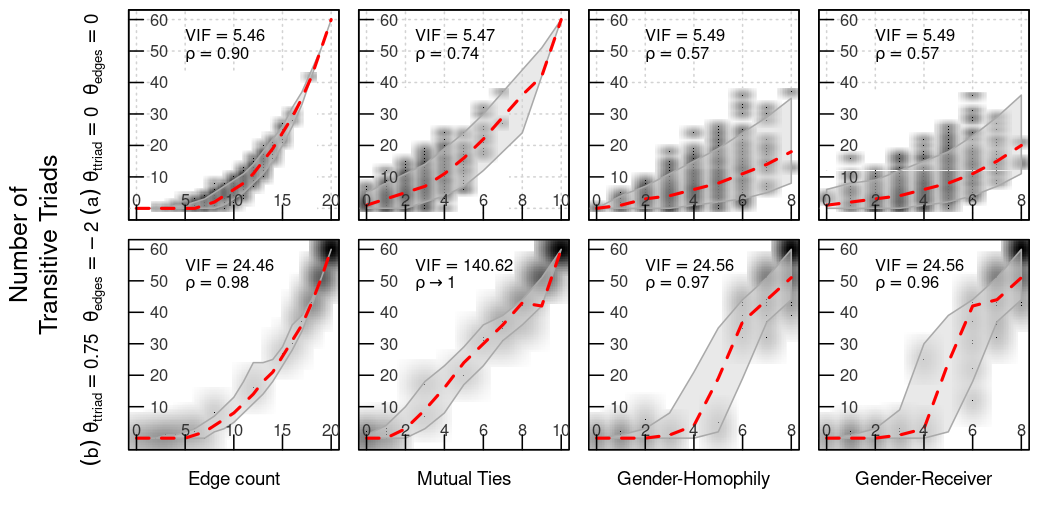
\includegraphics[width=0.8\textwidth,height=\textheight]{figures/conditional-prob-ttriad.png}

}

\end{figure}
\end{frame}

\begin{frame}{Collinearity in small networks}
\protect\hypertarget{collinearity-in-small-networks}{}
\begin{columns}[T]
\begin{column}{0.5\textwidth}
\begin{figure}

{\centering 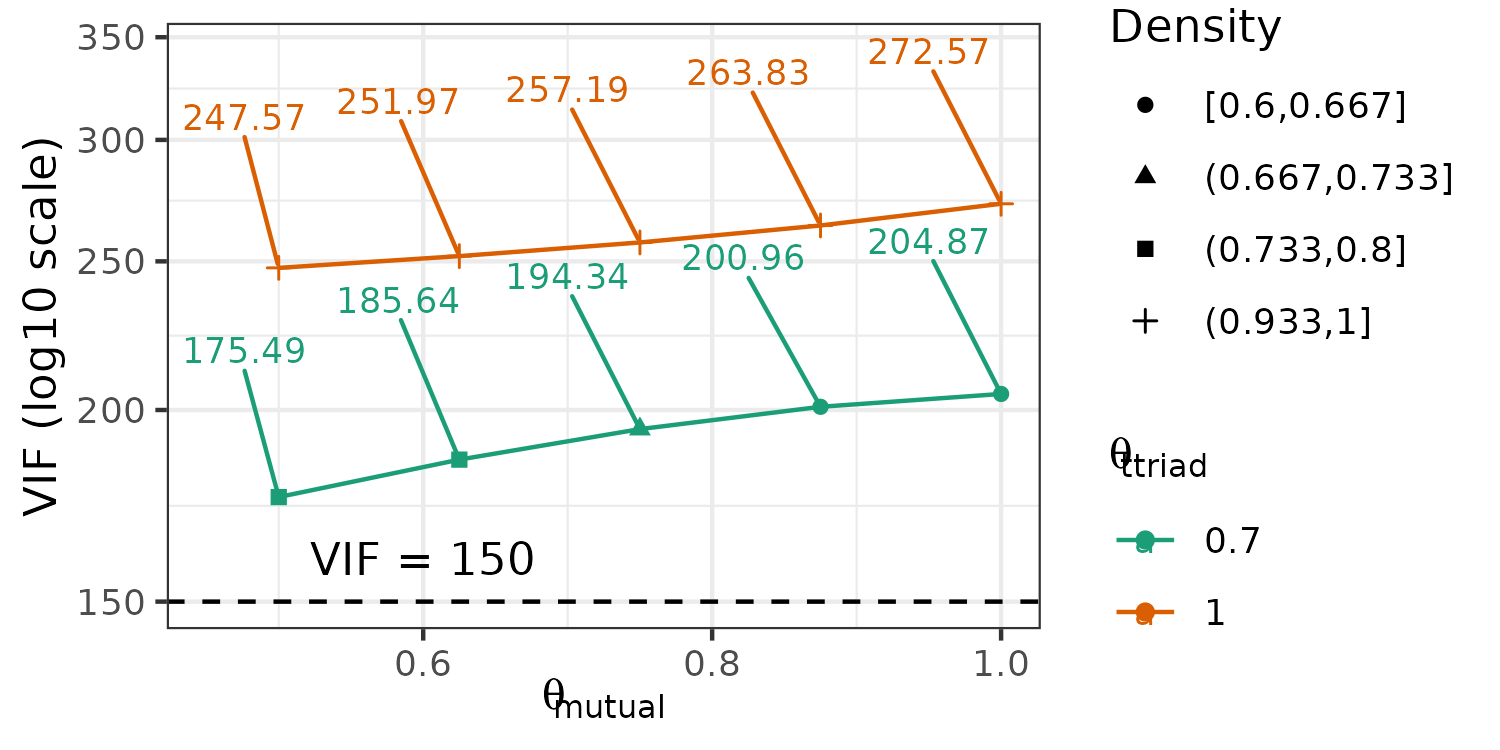
\includegraphics[width=0.9\textwidth,height=\textheight]{figures/vif-n=5.png}

}

\end{figure}
\end{column}

\begin{column}{0.5\textwidth}
\begin{figure}

{\centering 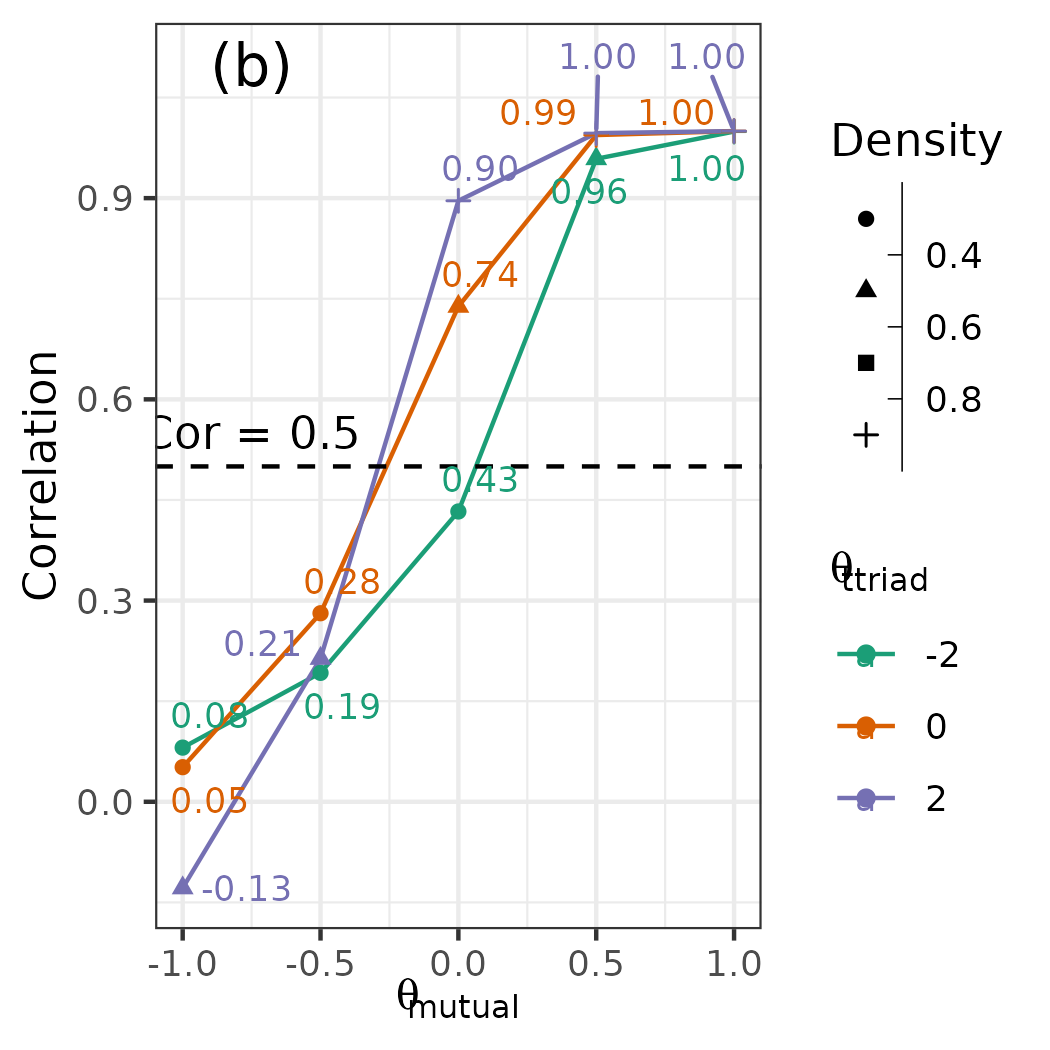
\includegraphics[width=0.9\textwidth,height=\textheight]{figures/cor-n=5.png}

}

\end{figure}
\end{column}
\end{columns}
\end{frame}

\begin{frame}{Discussion}
\protect\hypertarget{discussion}{}
A few questions:

\begin{itemize}
\item
  How would you address power analysis in ERGMs?
\item
  VIFs and correlations across statistics are significantly high in
  dense networks. How much do you think it matters? If it matters, how
  would you address it?
\item
  Relating both, is there any way in which a large sample size can help
  with collinearity?
\item
  In KCH, effect sizes are significantly large.
\item
  How much heterogeneity? Networks in KCH range from two to eight, but
  how about bigger samples? In Schweinberger, Krivitsky, and Butts
  (2017) it is mentioned the term ``comparative'', but there's no clear
  definition of what that means.
\end{itemize}
\end{frame}

\begin{frame}
\begin{block}{Thanks!}
\protect\hypertarget{thanks}{}
george.vegayon at utah.edu

\href{https://ggvy.cl}{\textbf{https://ggv.cl}}

\href{https://twitter.com/gvegayon}{\faIcon{twitter} @gvegayon}
\end{block}
\end{frame}

\begin{frame}{References}
\protect\hypertarget{references}{}
\hypertarget{refs}{}
\begin{CSLReferences}{1}{0}
\leavevmode\vadjust pre{\hypertarget{ref-duxburyDiagnosingMulticollinearityExponential2021}{}}%
Duxbury, Scott W. 2021. {``Diagnosing {Multicollinearity} in
{Exponential Random Graph Models}.''} \emph{Sociological Methods \&
Research} 50 (2): 491--530.
\url{https://doi.org/10.1177/0049124118782543}.

\leavevmode\vadjust pre{\hypertarget{ref-krivitskyTaleTwoDatasets2022}{}}%
Krivitsky, Pavel N., Pietro Coletti, and Niel Hens. 2022. {``A {Tale} of
{Two Datasets}: {Representativeness} and {Generalisability} of
{Inference} for {Samples} of {Networks}.''}

\leavevmode\vadjust pre{\hypertarget{ref-schweinbergerNoteRoleProjectivity2017}{}}%
Schweinberger, Michael, Pavel N. Krivitsky, and Carter T. Butts. 2017.
{``A Note on the Role of Projectivity in Likelihood-Based Inference for
Random Graph Models,''} July, 1--6.

\leavevmode\vadjust pre{\hypertarget{ref-schweinbergerExponentialFamilyModelsRandom2020}{}}%
Schweinberger, Michael, Pavel N. Krivitsky, Carter T. Butts, and
Jonathan R. Stewart. 2020. {``Exponential-{Family Models} of {Random
Graphs}: {Inference} in {Finite}, {Super} and {Infinite Population
Scenarios}.''} \emph{Statistical Science} 35 (4): 627--62.
\url{https://doi.org/10.1214/19-sts743}.

\end{CSLReferences}
\end{frame}



\end{document}
